% Preamble
\documentclass[../Relazione_circuiti]{subfiles}

% Packages

\graphicspath{{\subfix{../images/}}}

% Document
\begin{document}

\begin{wrapfigure}{r}{0.55\textwidth}

\end{wrapfigure}

\begin{minipage}{.44\textwidth}

  Per effettuare l'esperimento abbiamo utilizzato:
  \begin{itemize}
    \item Scheda Elvis II della National Instruments
    \item Computer
    % le ~ servono a non far andare a capo tra valore e unità di misura
    \item Due resistenze ($99.76 \pm 0.05$~\textOmega \hspace{1pt} su ramo Tweeter e $99.59 \pm 0.05$~\textOmega \hspace{1pt} su ramo Woofer), un condensatore ($1.03 \pm 0.01 $~\textmu F) e un'induttanza ($11.8 \pm 0.1$~mH)
  \end{itemize}

  La scheda millefori della Elvis ha fatto da base per il circuito, che è poi stato alimentato dal suo function
  generator, e tutte le misure sono state effettuate tramite il multimetro digitale e l'analog input multicanale sempre
  della Elvis (si veda l'appendice\,\ref{sec:errori_strumentali} per il calcolo delle incertezze su questi dati).\\
  Il computer si è interfacciato con la scheda per gestire le operazioni di misura. \\
  La componentistica elettrica è stata usata per realizzare il circuito.
\end{minipage}
\hfill
\begin{minipage}{0.55\textwidth}
  \centering
  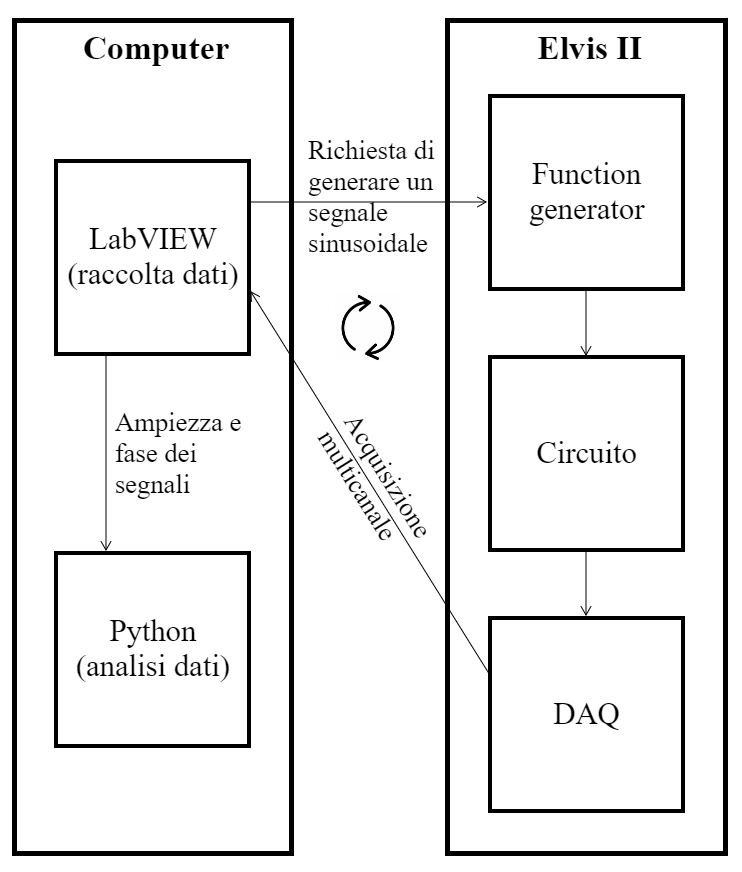
\includegraphics[width=.91\textwidth]{Pipeline_scheme.png}
  \captionof{figure}{\label{fig:schema_pipeline}Schema acquisizione bufferizzata}
\end{minipage}
È importante notare la bassa resistenza dell'induttanza utilizzata, trascurabile rispetto alle resistenze di carico
(circa $1$ \textOmega), necessaria per la validità di tutte le formule utilizzate in questo articolo.

\subsection{Misure effettuate}\label{subsec:misure-effettuate}

  Per misurare la resistenza interna del function generator della Elvis abbiamo messo una resistenza nota $R$ ai capi
  del generatore e misurato 299 volte la caduta di potenza su di essa, prendendo poi la media $V$, e calcolato
  \begin{equation*}
    Rg = R \left( \frac{ddp}{V} - 1 \right)
  \end{equation*}
  dove $ddp$ è la differenza di potenziale richiesta al generatore. \\

  \begin{wraptable}{r}{0.5\textwidth}
    \centering
    \begin{minipage}{0.43\textwidth}

      \centering
      \begin{tabular}{|c|c|}
        % Par name & Par val
        \hline
        Sample per buffer & 3000                           \\
        Sample al secondo & $ 450 \cdot 10^3 $                 \\
        Range             & 200 Hz − 10 kHz                \\
        Passo             & $\nu_{i+1} = \nu_i \cdot 1.01$ \\ \hline
      \end{tabular}

      \captionof{table}{Parametri per acquisizioni bufferizate}
      \label{tab:parametri-daq}

    \end{minipage}

  \end{wraptable}

%  Abbiamo poi impostato l'acquisizione dati
%  a 3000~sample a $ 450 \cdot 10^3 $~sample/s su un range da 200~Hz a
%  20~kHz, con un passo tale da essere costante in scala logaritmica (ovvero $ \nu_{i+1} = \nu_i \cdot 1.01 $),
  Abbiamo poi impostato l'acquisizione dati come in Tab\,\ref{tab:parametri-daq} e con questi parametri abbiamo
  misurato:
  \begin{itemize}
    \item La differenza di potenziale tra il generatore e il ground
    \item La caduta di potenziale sulle resistenze di carico
  \end{itemize}

  Da questi dati abbiamo estratto con un fit della forma $ A \sin\left( \omega t + \phi \right) $ i valori di ampiezza e
  fase (come frequenza abbiamo usato quella del function generator, nota con un'incertezza assoluta di 0.186 Hz), che
  abbiamo utilizzato nella fase di analisi (Si veda la Fig.\,\ref{fig:schema_pipeline} per uno schema del processo
  descritto)

%  Abbiamo poi misurato l'ampiezza del segnale su entrambi i canali in funzione della frequenza, riferita al ground del
%  circuito.
%
%  La fase invece è stata misurata rispetto al canale Woofer.
%  Si ha quindi che la fase del Tweeter rispetto al Woofer rappresenta in realtà la differenza di fase tra i due
%    riferita
%  al generatore, ed è definita come nell'Eq.\,\eqref{eq:p_diff}.
%
%  Ampiezza e fase sono stati estratti tramite un fit sinusoidale della forma $ A \sin\left( \omega t + \phi \right) $
%  su delle acquisizioni da 3000 sample a $ 450 \cdot 10^3 $ sample/s su un range da 200 Hz a 20 kHz, con un passo tale
%  da essere costante in scala logaritmica, ovvero $ \nu_{i+1} = \nu_i \cdot 1.01 $

\end{document}